\documentclass[11pt,a4paper]{article}  % Déclare la classe du document.

\newcommand{\chaptermark}[2]{\og #2 \fg{} (#1)} % ligne uniquement pour éviter une erreur en cas d'article
\usepackage[table,dvipsnames,svgnames]{xcolor}
\usepackage{listingsutf8}
%\usepackage[utf8]{inputenc}% gestion des accents (source)
\usepackage[T1]{fontenc}% gestion des accents (PDF)
\usepackage{fontspec}
\usepackage[french]{babel}% gestion du français
\usepackage{textcomp}% caractères additionnels
\usepackage{mathtools,amssymb,amsthm}% packages de l'AMS + mathtools
\usepackage{amsmath}
\usepackage{yhmath}
\usepackage{mathpazo}
\usepackage[scaled=0.95]{helvet}
\usepackage{courier}
%\usepackage{fourier}
%\usepackage[scaled=0.95]{helvet}
%\usepackage{courier}
\usepackage{bm}
\usepackage{gensymb}
\usepackage{graphicx}

\usepackage{enumitem}
\usepackage{pifont}

\usepackage{pstricks}
\usepackage{pstricks-add}
\usepackage{pst-eucl}
\usepackage{pgfplots}
\let\clipbox\relax
%\usepackage{pst-plot,pst-text,pst-tree,pstricks-add}
%\usepackage{pst-node} % required package
\usepackage{pst-all}
\usepackage[most,skins,breakable]{tcolorbox}

\usepackage{euscript}





% ############### Nouvelles commandes ###############
% Coloration des labels des points dans pst-eucl
\makeatletter
\define@key[psset]{pst-eucl}{LabelColor}{\def\psk@LabelColor{#1}}
\psset{LabelColor=black}
\def\Pst@WhichLabel#1{{\color{\psk@LabelColor}%
		\ifx\psk@PointName\@default#1\else\psk@PointName\fi}}
\makeatother

% renomme le symbole #2 en #1#2 et invalide le symbole initial #2:
\def\renamesymbol#1#2{
	\expandafter\let\expandafter\newsym\expandafter=\csname#2\endcsname
	\expandafter\global\expandafter\let\csname#1#2\endcsname=\newsym
	\expandafter\global\expandafter\let\csname#2\endcsname=\origsym
}



\usepackage{ProfCollege}
\renamesymbol{Casio}{Calculatrice}
\usepackage[nonshellescape]{ProfLycee}



%\usepackage[left=1.5cm,right=1.5cm,top=2.5cm,bottom=2.5cm]{geometry}
\usepackage[left=13mm,right=13mm,top=18mm,bottom=18mm,footskip=30pt]{geometry}
\setlength{\headheight}{15pt}

\usepackage{titlesec}
\usepackage{pas-math}
\usepackage{longtable}
\usepackage{tikz,tkz-tab}
\usepackage{amsmath}
\usepackage[right]{eurosym}
\usepackage{sectsty}
\usepackage{tipfr}
\usepackage{setspace}

%pour faire les touches de la calculatrices
\usepackage{menukeys}
\renewmenumacro{\menu}{roundedmenus} % default: menus
\renewmenumacro{\directory}{pathswithfolder} % default: paths
\renewmenumacro{\keys}{shadowedroundedkeys} % default: roundedkeys


\usepackage{multicol}
\usepackage{multirow}
\usepackage{systeme}

%% Format des titres de chapitres, paragraphes, ...
\titleformat{\chapter}[frame]
{\color{red!85!white}\normalsize}%
{\filright\sffamily\Large%
	\enspace Chapitre \thechapter\enspace}%
{8pt}
{\color{red!85!white}\rule{0pt}{30pt}\sffamily\Huge\bfseries\filcenter}
%%%%%%%%%%%%%%%%%%%%
\titlespacing{\chapter}{0pc}{0pc}{2pc}
\titlespacing{\subsection}{2pc}{}{}

\titleformat{\subsection}[block]{\hspace{1em}}{\thesubsection}{1em .}{}
\titleformat{\subsubsection}[block]{\hspace{2em}}{\thesubsection}{1em )}{}

\chapterfont{\color{red}{}}
\sectionfont{\color{green!55!black}{}}
\subsectionfont{\color{cyan!65!black}{}}
\subsubsectionfont{\color{violet}{}}
\renewcommand{\thesection}{\color{green!55!black}\Roman{section}.}
\renewcommand{\thesubsection}{\color{cyan!65!black}\arabic{subsection})}
\renewcommand{\thesubsubsection}{\color{violet}\alph{subsubsection})}
\setcounter{secnumdepth}{3}

\titleformat{\subsection}[block]{\hspace{1em}}{\thesubsection}{1em .}{}
\titleformat{\subsubsection}[block]{\hspace{2em}}{\thesubsection}{1em )}{}

\usepackage[column=A]{cellspace}
\setlength{\cellspacebottomlimit}{4pt}
\setlength{\cellspacetoplimit}{4pt}
\setlength{\parindent}{2pt}
\setlength{\tabcolsep}{0.5cm}


%entête et pieds de pages
\usepackage{fancyhdr}
\pagestyle{fancy}
\fancyhf{}
\usepackage{lastpage}
\renewcommand{\chaptermark}[1]{\markboth {Chap. \thechapter~ - ~#1}{}}
\renewcommand\headrulewidth{1pt}
\fancyhead[LO,RE]{1ère G - spécialité maths}
\fancyhead[RO,LE]{\leftmark}
\renewcommand\footrulewidth{1pt}
\fancyfoot[LO,RE]{Année 2025-2026}
\fancyfoot[RO,LE]{\textbf{Page \thepage/\pageref{LastPage}}}

%Mes boites pour les définitions, propriétés, remarques, ...

%Mes boites pour les définitions, propriétés, remarques, ...

\newcommand\titrebox[1]{\textbf{#1}}
\newtcolorbox{definition}{breakable,colback=red!10!white,
	colframe=red!85!white, fonttitle=\bfseries,enhanced,
	attach boxed title to top left={xshift=5mm, yshift=-2mm},boxed title style={size=small,colback=red!10!white,colframe=red!85!white, arc=0.5mm},
	title=\textcolor{red!85!white}{Définition} , arc=3mm}

\newtcolorbox{definitionTitre}[1]{breakable,colback=red!10!white,
	colframe=red!85!white, fonttitle=\bfseries,enhanced,
	attach boxed title to top left={xshift=5mm, yshift=-2mm},boxed title style={size=small,colback=red!10!white,colframe=red!85!white, arc=0.5mm},
	title=\textcolor{red!85!white}{Définition - #1} , arc=3mm}

\newtcolorbox{definitionPerso}[1]{breakable,colback=red!10!white,
	colframe=red!85!white, fonttitle=\bfseries,enhanced,
	attach boxed title to top left={xshift=5mm, yshift=-2mm},boxed title style={size=small,colback=red!10!white,colframe=red!85!white, arc=0.5mm},
	title=\textcolor{red!85!white}{#1} , arc=3mm}

\newtcolorbox{regle}{breakable,colback=red!10!white,
	colframe=red!85!white, fonttitle=\bfseries,enhanced,
	attach boxed title to top left={xshift=5mm, yshift=-2mm},boxed title style={size=small,colback=red!10!white,colframe=red!85!white, arc=0.5mm},
	title=\textcolor{red!85!white}{Règle} , arc=3mm}

\newtcolorbox{regles}{breakable,colback=red!10!white,
	colframe=red!85!white, fonttitle=\bfseries,enhanced,
	attach boxed title to top left={xshift=5mm, yshift=-2mm},boxed title style={size=small,colback=red!10!white,colframe=red!85!white, arc=0.5mm},
	title=\textcolor{red!85!white}{Règles} , arc=3mm}

\newtcolorbox{definitions}{breakable,colback=red!10!white,
	colframe=red!85!white, fonttitle=\bfseries,enhanced,
	attach boxed title to top left={xshift=5mm, yshift=-2mm},boxed title style={size=small,colback=red!10!white,colframe=red!85!white, arc=0.5mm},
	title=\textcolor{red!85!white}{Définitions} , arc=3mm}

\newtcolorbox{propriete}{breakable,colback=red!10!white,
	colframe=red!85!white, fonttitle=\bfseries,enhanced,
	attach boxed title to top left={xshift=5mm, yshift=-2mm},boxed title style={size=small,colback=red!10!white,colframe=red!85!white, arc=0.5mm},
	title=\textcolor{red!85!white}{Propriété} , arc=3mm}

\newtcolorbox{proprieteTitre}[1]{breakable,colback=red!10!white,
	colframe=red!85!white, fonttitle=\bfseries,enhanced,
	attach boxed title to top left={xshift=5mm, yshift=-2mm},boxed title style={size=small,colback=red!10!white,colframe=red!85!white, arc=0.5mm},
	title=\textcolor{red!85!white}{Propriété - #1} , arc=3mm}

\newtcolorbox{proprietes}{breakable,colback=red!10!white,
	colframe=red!85!white, fonttitle=\bfseries,enhanced,
	attach boxed title to top left={xshift=5mm, yshift=-2mm},boxed title style={size=small,colback=red!10!white,colframe=red!85!white, arc=0.5mm},
	title=\textcolor{red!85!white}{Propriétés} , arc=3mm}

\newtcolorbox{theoreme}{breakable,colback=red!10!white,
	colframe=red!85!white, fonttitle=\bfseries,enhanced,
	attach boxed title to top left={xshift=5mm, yshift=-2mm},boxed title style={size=small,colback=red!10!white,colframe=red!85!white, arc=0.5mm},
	title=\textcolor{red!85!white}{Théorème} , arc=3mm}

\newtcolorbox{theoremeTitre}[1]{breakable,colback=red!10!white,
	colframe=red!85!white, fonttitle=\bfseries,enhanced,
	attach boxed title to top left={xshift=5mm, yshift=-2mm},boxed title style={size=small,colback=red!10!white,colframe=red!85!white, arc=0.5mm},
	title=\textcolor{red!85!white}{Théorème - #1} , arc=3mm}

\newtcolorbox{theoremes}{breakable,colback=red!10!white,
	colframe=red!85!white, fonttitle=\bfseries,enhanced,
	attach boxed title to top left={xshift=5mm, yshift=-2mm},boxed title style={size=small,colback=red!10!white,colframe=red!85!white, arc=0.5mm},
	title=\textcolor{red!85!white}{Théorèmes} , arc=3mm}

\newtcolorbox{bexemple}{
	enhanced,
	breakable,
	fonttitle=\bfseries,
	frame empty,
	nobeforeafter,
	borderline west={0.5mm}{0mm}{cyan!75!black},
	title=\textcolor{cyan!75!black}{\faHubspot\:\:Exemple},
	%title after break=Exemple (suite),
	colback=white,
	extras={enhanced, frame empty},
	detach title,before upper={\tcbtitle\ :\quad },
}

\newtcolorbox{bexemples}{
	enhanced,
	breakable,
	fonttitle=\bfseries,
	frame empty,
	nobeforeafter,
	borderline west={0.5mm}{0mm}{cyan!75!black},
	title=\textcolor{cyan!75!black}{\faHubspot\:\:Exemples},
	%title after break=Exemples (suite),
	colback=white,
	extras={enhanced, frame empty},
	detach title,before upper={\tcbtitle\ :\quad },
}

\newtcolorbox{bexemplet}[1]{
	enhanced,
	breakable,
	fonttitle=\bfseries,
	frame empty,
	borderline west={0.5mm}{0mm}{cyan!75!black},
	title=\textcolor{cyan!75!black}{\faHubspot\:\:Exemple - #1},
	colback=white,
	extras={enhanced, frame empty},
	detach title,before upper={\tcbtitle\ :\quad },
}

\newtcolorbox{brmq}{
	enhanced,
	breakable,
	fonttitle=\bfseries,
	frame empty,
	nobeforeafter,
	borderline west={0.5mm}{0mm}{orange!95!white},
	title=\textcolor{orange!85!white}{\faHandPointRight[regular]\:\:Remarque} ,
	colback=white,
	extras={enhanced, frame empty},
	detach title,before upper={\tcbtitle\ \quad },
}

\newtcolorbox{brmqs}{
	enhanced,
	breakable,
	fonttitle=\bfseries,
	frame empty,
	nobeforeafter,
	borderline west={0.5mm}{0mm}{orange!85!white},
	title=\textcolor{orange!85!white}{\faHandPointRight[regular]\:\:Remarques},
	colback=white,
	detach title,before upper={\tcbtitle\ \quad },
	extras={enhanced, frame empty},
}

\newtcolorbox{brmqt}[1]{
	enhanced,
	breakable,
	fonttitle=\bfseries,
	frame empty,
	nobeforeafter,
	borderline west={0.5mm}{0mm}{orange!85!white},
	title=\textcolor{orange!85!white}{\faHandPointRight[regular]\:\:Remarque - #1},
	colback=white,
	extras={enhanced, frame empty},
	detach title,before upper={\tcbtitle\ \quad },
}

\newtcolorbox{consequences}[1]{
	enhanced,
	breakable,
	fonttitle=\bfseries,
	frame empty,
	nobeforeafter,
	borderline west={0.5mm}{0mm}{ProcessBlue},
	title=\textcolor{ProcessBlue}{#1},
	colback=white,
	extras={enhanced, frame empty},
	detach title,before upper={\tcbtitle\ :\quad },
}

\newtcolorbox{bmethode}{
	enhanced,
	breakable,
	fonttitle=\bfseries,
	frame empty,
	nobeforeafter,
	borderline west={0.5mm}{0mm}{blue!75!black},
	title=\textcolor{blue!75!black}{Méthode} ,
	colback=white,
	extras={enhanced, frame empty},
	attach boxed title to top left = {xshift = -3mm},
	boxed title style={size=small,colback=white,colframe=blue!75!black, arc=3mm,
	}
}

\newtcolorbox{bmethodes}{
	enhanced,
	breakable,
	fonttitle=\bfseries,
	frame empty,
	nobeforeafter,
	borderline west={0.5mm}{0mm}{blue!75!black},
	title=\textcolor{blue!75!black}{Méthodes} ,
	colback=white,
	extras={enhanced, frame empty},
	attach boxed title to top left = {xshift = -3mm},
	boxed title style={size=small,colback=blue!75!black,colframe=blue!75!black, arc=3mm,
	}
	boxed title after break style={size=small,colback=white,colframe=blue!75!black, arc=3mm,
	}
}

\newtcolorbox{bmethodet}[1]{
	enhanced,
	breakable,
	fonttitle=\bfseries,
	frame empty,
	nobeforeafter,
	borderline west={0.5mm}{0mm}{blue!75!black},
	title=\textcolor{blue!75!black}{\faTasks\:\:Méthode - #1} ,
	colback=white,
	extras={enhanced, frame empty},
	attach boxed title to top left = {xshift = -3mm},
	boxed title style={size=small,colback=white,colframe=blue!75!black, arc=3mm,
	}
}

\newtcolorbox{bdemo}{
	enhanced,
	breakable,
	fonttitle=\bfseries,
	frame empty,
	nobeforeafter,
	borderline west={0.5mm}{0mm}{violet!65!white},
	title={\faEdit[regular]\:\:Démonstration},
	%title after break=Démonstration (suite),
	colback=white,
	extras={enhanced, frame empty},
	attach boxed title to top left = {xshift = -3mm},
	boxed title style={size=small,colback=violet!65!white,colframe=violet!65!white, arc=3mm,
	}
}

\newtcolorbox{bdemos}{
	enhanced,
	breakable,
	fonttitle=\bfseries,
	frame empty,
	nobeforeafter,
	borderline west={0.5mm}{0mm}{violet!65!white},
	title={\faEdit[regular]\:\:Démonstrations},
	%title after break=Démonstration (suite),
	colback=white,
	extras={enhanced, frame empty},
	attach boxed title to top left = {xshift = -3mm},
	boxed title style={size=small,colback=violet!65!white,colframe=violet!65!white, arc=3mm,
	}
}

\newtcolorbox{bdemot}[1]{
	enhanced,
	breakable,
	fonttitle=\bfseries,
	frame empty,
	nobeforeafter,
	borderline west={0.5mm}{0mm}{violet!65!white},
	title={\faEdit[regular]\:\:Démonstration - #1},
	%title after break=Démonstration (suite),
	colback=white,
	extras={enhanced, frame empty},
	attach boxed title to top left = {xshift = -3mm},
	boxed title style={size=small,colback=violet!65!white,colframe=violet!65!white, arc=3mm,
	}
}

\newtcolorbox{boxPerso}[2]{
	enhanced,
	breakable,
	fonttitle=\bfseries,
	frame empty,
	nobeforeafter,
	borderline west={0.5mm}{0mm}{#2},
	title=#1,
	%title after break=Exemple (suite),
	colback=white,
	extras={enhanced, frame empty},
	detach title,before upper={\tcbtitle\ :\quad },
}


\newcommand*{\Coord}[3]{% 
	\ensuremath{\vv{#1}\, 
		\begin{pmatrix} 
			#2\\ 
			#3 
\end{pmatrix}}}

\newcommand*{\CoordSV}[2]{% 
	\ensuremath{\begin{pmatrix} 
			#1\\ 
			#2 
\end{pmatrix}}}

\newcommand*{\Coordp}[3]{% 
	\ensuremath{\vv{#1}\, 
		\left\lvert 
		\begin{matrix} 
			#2\\ 
			#3 
		\end{matrix}  
		\right.% Ne pas oublier le délimiteur invisible. 
}}


%personnalisation des listes non numérotées pour les différentes boites 
\newlist{itemEx}{itemize}{2}
\setlist[itemEx,1]{label=$\bullet$, font=\color{cyan!75!black}}
\setlist[itemEx,2]{label=$\bullet$, font=\color{cyan!75!black}}

\newlist{enumEx}{enumerate}{2}
\setlist[enumEx,1]{label=\arabic*), font=\bf\color{cyan!75!black}}
\setlist[enumEx,2]{label=\alph*), font=\bf\color{cyan!75!black}}

\newlist{itemMet}{itemize}{2}
\setlist[itemMet,1]{label=$\bullet$, font=\color{blue!75!black}}
\setlist[itemMet,2]{label=$\bullet$, font=\color{blue!75!black}}

\newlist{enumMet}{enumerate}{2}
\setlist[enumMet,1]{label=\arabic*), font=\bf\color{blue!75!black}}
\setlist[enumMet,2]{label=\alph*), font=\bf\color{blue!75!black}}

\newlist{itemDef}{itemize}{2}
\setlist[itemDef,1]{label=$\bullet$, font=\color{ForestGreen}}
\setlist[itemDef,2]{label=$\bullet$, font=\color{ForestGreen}}

\newlist{enumDef}{enumerate}{2}
\setlist[enumDef,1]{label=\arabic*), font=\bf\color{ForestGreen}}
\setlist[enumDef,2]{label=\alph*), font=\bf\color{ForestGreen}}

\newlist{itemProp}{itemize}{2}
\setlist[itemProp,1]{label=$\bullet$, font=\color{red!85!white}}
\setlist[itemProp,2]{label=$\bullet$, font=\color{red!85!white}}

\newlist{enumProp}{enumerate}{2}
\setlist[enumProp,1]{label=\arabic*), font=\bf\color{red!85!white}}
\setlist[enumProp,2]{label=\alph*), font=\bf\color{red!85!white}}

\newlist{itemDem}{itemize}{2}
\setlist[itemDem,1]{label=$\bullet$, font=\color{violet!85!white}}
\setlist[itemDem,2]{label=$\bullet$, font=\color{violet!85!white}}

\newlist{enumDem}{enumerate}{2}
\setlist[enumDem,1]{label=\arabic*), font=\bf\color{violet!85!white}}
\setlist[enumDem,2]{label=\alph*), font=\bf\color{violet!85!white}}

\newlist{itemRem}{itemize}{2}
\setlist[itemRem,1]{label=\ding{43}, font=\color{orange!85!white}}
\setlist[itemRem,2]{label=\ding{43}, font=\color{orange!85!white}}

\newlist{enumRem}{enumerate}{2}
\setlist[enumRem,1]{label=\arabic*), font=\bf\color{orange!85!white}}
\setlist[enumRem,2]{label=\alph*), font=\bf\color{orange!85!white}}

% nouvelle commande pour mettre entre guillemets une expression
\newcommand{\guillemets}[1]{\og \emph{#1} \fg}


\newcommand{\corr}[1]{\fcolorbox{red}{yellow!30}{#1}}

\newtcolorbox{corrBox}{enhanced,breakable,boxrule=1pt,nobeforeafter,boxsep=0pt,left=\fboxsep,right=\fboxsep,colback=yellow!30,colframe=red!75!black}

% commandes pour mettre en couleur (et en gras) dans une expression mathématique.
\newcommand{\mVert}[1]{{\color{green!55!black}\bm{#1}}}
\newcommand{\mVertWB}[1]{{\color{green!55!black}#1}}
\newcommand{\mRouge}[1]{{\color{red!85!white}\bm{#1}}}
\newcommand{\mRougeWB}[1]{{\color{red!85!white}#1}}
\newcommand{\mBleu}[1]{{\color{blue!75!black}\bm{#1}}}
\newcommand{\mBleuWB}[1]{{\color{blue!75!black}#1}}
\newcommand{\mOrange}[1]{{\color{orange!75!white}\bm{#1}}}
\newcommand{\mOrangeWB}[1]{{\color{orange!75!white}#1}}
\newcommand{\mViolet}[1]{{\color{violet!85!white}\bm{#1}}}
\newcommand{\mVioletWB}[1]{{\color{violet!85!white}#1}}

%commandes pour les flèches de distributivité.
\newcommand{\tikzmarkBB}[2][]{ \tikz[remember picture, overlay, baseline=-0.5ex]\node[#1, left](#2){}; }
\newcommand{\flechePropV}[4][]{ \tikz[remember picture, overlay]\draw (#2)edge[bend left=90,min distance=1em, -stealth]node[midway, #1]{#4}(#3); }
\newcommand{\flechePropH}[4][]{ \tikz[remember picture, overlay]\draw (#2)edge[bend left=90, min distance=1em, -stealth]node[midway, #1]{#4}(#3); }
\newcommand{\flechePropHbas}[4][]{ \tikz[remember picture, overlay]\draw (#2)edge[bend left=-90, min distance=1em, -stealth]node[midway, #1]{#4}(#3); }


\lstdefinestyle{algo}{%
	inputencoding=utf8,
	mathescape,
	basicstyle=\footnotesize\ttfamily,
	numberstyle=\scriptsize\ttfamily\color{gray},
	showstringspaces=false,
	tabsize=2,
	numbers=left,
	framexleftmargin=8mm,
	xleftmargin=8mm,
	keepspaces=true,
	frame=lines,
	framerule=1pt,
	rulecolor=\color{green!50!black},
	backgroundcolor=\color{green!5},
	keywords = {Pour, allant, Si, alors, Sinon, Fin},    
	morecomment=[l][commentstyle]{//},
	commentstyle=\color{gray},
	classoffset=0,
	keywordstyle=\color{blue!75},
	classoffset=1,
	morekeywords = {Afficher},
	keywordstyle=\color{green!50!black},
	classoffset=0,
	morestring=[b]",
	stringstyle=\color{red!75},
	literate=
	{é}{{\'e}}{1}%
	{è}{{\`e}}{1}%
	{à}{{\`a}}{1}%
	{â}{{\^a}}{1}%%%
	{ç}{{\c{c}}}{1}%
	{œ}{{\oe}}{1}%
	{ù}{{\`u}}{1}%
	{É}{{\'E}}{1}%
	{È}{{\`E}}{1}%
	{À}{{\`A}}{1}%
	{Ç}{{\c{C}}}{1}%
	{Œ}{{\OE}}{1}%
	{Ê}{{\^E}}{1}%
	{ê}{{\^e}}{1}%
	{î}{{\^i}}{1}%
	{ï}{{\"i}}{1}%%%
	{ô}{{\^o}}{1}%
	{û}{{\^u}}{1}%
	{=}{$\leftarrow$}{1}%
	{==}{$={}$}{1}}


%  --------   Macro pour les exercices et leur numérotation  

\newcounter{exo}

\setcounter{exo}{1}

\newcommand{\exercice}[1]{\vskip 0.2cm\noindent{\bf \ Exercice \theexo {  #1 }}\addtocounter{exo}{1}}

\newcounter{rit}

\setcounter{rit}{1}

\newcommand{\rituel}[1]{\vskip 0.2cm\noindent{ \bf \ \underline{Rit. \therit {  #1 }}}\addtocounter{rit}{1}}

\newcommand{\raisedrule}[2][0em]{\leaders\hbox{\rule[#1]{1pt}{#2}}\hfill}

\newcounter{numexo}

\setcounter{numexo}{1}

\newcommand{\exerciceDS}[1]{\vskip 0.6cm\noindent\rule[+2pt]{1cm}{0.5pt}\ {\large\bf \ Exercice \thenumexo {  #1 }}\raisedrule[+2pt]{0.5pt}\null\addtocounter{numexo}{1}\par\vskip 0,4cm}

\newcommand{\bareme}[1]{\tikz\node[circle,draw,inner sep=1pt,outer sep=1pt, color=red]{\textbf{#1}};}

%  --------   Pour le langage Python

% Default fixed font does not support bold face
\DeclareFixedFont{\ttb}{T1}{txtt}{bx}{n}{12} % for bold
\DeclareFixedFont{\ttm}{T1}{txtt}{m}{n}{12}  % for normal

% Custom colors
\usepackage{color}
\definecolor{deepblue}{rgb}{0,0,0.5}
\definecolor{deepred}{rgb}{0.6,0,0}
\definecolor{deepgreen}{rgb}{0,0.5,0}

\usepackage{listings}

% Python style for highlighting
\newcommand\pythonstyle{\lstset{
		language=Python,
		basicstyle=\ttm,
		otherkeywords={self},             % Add keywords here
		keywordstyle=\ttb\color{deepblue},
		emph={MyClass,__init__},          % Custom highlighting
		emphstyle=\ttb\color{deepred},    % Custom highlighting style
		stringstyle=\color{deepgreen},
		frame=tb,                         % Any extra options here
		showstringspaces=false            % 
}}


% Python environment
\lstnewenvironment{python}[1][]
{
	\pythonstyle
	\lstset{#1}
}
{}

% Python for external files
\newcommand\pythonexternal[2][]{{
		\pythonstyle
		\lstinputlisting[#1]{#2}}}

% Python for inline
\newcommand\pythoninline[1]{{\pythonstyle\lstinline!#1!}}


% \begin{document}
	
	% \section{``In-text'' listing highlighting}
	
	% \begin{python}
		% class MyClass(Yourclass):
		%     def __init__(self, my, yours):
		%         bla = '5 1 2 3 4'
		%         print bla
		% \end{python}
	
	% \section{External listing highlighting}
	
	% \pythonexternal{demo.py}
	
	% \section{Inline highlighting}
	
	% Definition \pythoninline{class MyClass} means \dots
	
	% \end{document}

\definecolor{codegreen}{rgb}{0,0.6,0}
\definecolor{codegray}{rgb}{0.5,0.5,0.5}
\definecolor{codepurple}{rgb}{0.58,0,0.82}
\definecolor{backcolour}{rgb}{0.95,0.95,0.92}

\lstdefinestyle{myStyle}{
	backgroundcolor=\color{backcolour},   
	commentstyle=\color{codegreen},
	keywordstyle=\color{magenta},
	numberstyle=\tiny\color{codegray},
	stringstyle=\color{codepurple},
	basicstyle=\ttfamily\footnotesize,
	breakatwhitespace=false,         
	breaklines=true,                 
	captionpos=b,                    
	keepspaces=true,                 
	numbers=left,                    
	numbersep=5pt,                  
	showspaces=false,                
	showstringspaces=false,
	showtabs=false,                  
	tabsize=2
}

\lstset{style=myStyle}

\newcommand{\normeB}[1]{\left\Vert \vv{#1}\right\Vert}

\newcommand\grasmaths[1]{\symbf{#1}}
\newcommand\sfbmath[1]{\symbf{\symsfup{#1}}}
\definecolor{marron}{rgb}{0.64,0.16,0.16}
\definecolor{titrebleu}{rgb}{0,0,0.6}

\usepackage{tabularx}
\usepackage{wasysym}
% ===========================tableaux de base
\newcolumntype{R}[1]{>{\raggedleft\arraybackslash }b{#1}} 
\newcolumntype{L}[1]{>{\raggedright\arraybackslash }b{#1}}
\newcolumntype{C}[1]{>{\centering\arraybackslash }b{#1}}
\newcolumntype{M}[1]{>{\centering\arraybackslash }m{#1}} %doublecentrée
\renewcommand{\tabularxcolumn}[1]{m{#1}}
\newcolumntype{Y}{>{\centering\arraybackslash }X}

%=============================boîtes de cours
\usepackage{fontawesome5}
\newcommand\fontbox{\sffamily}
%\newcommand\titrebox[1]{\textbf{#1}}
\tcbuselibrary{breakable}
\tcbset{bdefaut/.style={%
		fonttitle=\fontbox,%
		enhanced,breakable,center,boxrule=1.25pt,drop shadow=black!33!white,%
		sharp corners=uphill,arc=12pt,before skip=12pt,after skip=12pt,%
		left=5pt,leftupper=5pt,top=1mm,bottom=1mm,%
		before upper=\leavevmode
	}
}
\NewDocumentCommand\bbnewbox{ m m m m O{#4} !O{} }{%nom + titre + icone + bordure/titre/fondtitre + couleur fond + options
	\DeclareTColorBox{#1}{ O{} }{%
		bdefaut,%
		colframe=#4,coltitle=#4!25!Black,colbacktitle=#4!35,colback=#5!10,%
		title={#3\:\:\titrebox{#2##1}},%
		#6
	}%
}

\bbnewbox{bdefi}{Définition}{\faIcon[regular]{comment-dots}}{ForestGreen}
\bbnewbox{bcor}{Corollaire}{\faIcon[regular]{comment-dots}}{ForestGreen}
\bbnewbox{bdefis}{Définitions}{\faIcon[regular]{comment-dots}}{ForestGreen}
\bbnewbox{bhumour}{Humour}{\faIcon[regular]{laugh-wink}}{Yellow}
%\bbnewbox{bprop}{Propriété}{\faCog}{Salmon}
\bbnewbox{bprop}{Propriété}{\faCog}{red!85!white}
\bbnewbox{bprops}{Propriétés}{\faCog}{Salmon}
\bbnewbox{bcscq}{Conséquence}{\faArrowAltCircleRight[regular]}{Salmon}
\bbnewbox{bthm}{Théorème}{\faBullhorn}{FireBrick}
\bbnewbox{blog}{Logiciel}{\faDev}{CornflowerBlue}[white]
\bbnewbox{bhistoire}{Point histoire}{\faUniversity}{Chocolate}[white]

%\bbnewbox{brmq}{Remarque}{\faHandPointRight[regular]}{MidnightBlue}[white]
\bbnewbox{bexercice}{Exercice}{\faHubspot}{MidnightBlue}
%\bbnewbox{bexemple}{Exemple}{\faHubspot}{MediumTurquoise}
\bbnewbox{bvoc}{Vocabulaire}{\faList*[regular]}{YellowGreen}
\bbnewbox{bnota}{Notation}{\faList*}{YellowGreen}
\bbnewbox{bregle}{Règle}{\faList*}{YellowGreen}
\bbnewbox{bcadre}{Cadre}{\faInfoCircle}{Peru}
\bbnewbox{bidee}{Idée}{\faInfo}{LightBlue}
\bbnewbox{bintro}{Intro}{\faMarker}{LightSalmon}
\bbnewbox{billustr}{Illustration}{\faChartLine}{Crimson}[White]
\bbnewbox{bvideo}{}{\faIcon[regular]{file-video}}{teal}[White]
\bbnewbox{bbilan}{Bilan}{\faForward}{Purple}
%\bbnewbox{bmethode}{Méthode}{\faTasks}{Coral}
%\bbnewbox{bmethode}{Méthode}{\faTasks}{blue!75!black}
\bbnewbox{btuto}{Tuto}{\faTerminal}{Coral}[White]
\bbnewbox{bmanip}{Manipulation}{\faCodeBranch}{DarkCyan}[White]
\bbnewbox{bcalco}{Calculatrice}{\faCalculator}{MediumVioletRed}[White]
\bbnewbox{boutil}{Outil}{\faTools}{DeepSkyBlue}[White]
\bbnewbox{basavoir}{À savoir}{\faHeart}{Red}
\bbnewbox{bbloctd}{TD}{\faHourglassStart}{LightSeaGreen}[White]
\bbnewbox{bblocdm}{À vous de jouer}{\faHourglassStart}{LightSeaGreen}[White]
%\bbnewbox{brappel}{Rappel}{\faHandPointUp[regular]}{LightSalmon}
\bbnewbox{brappel}{Rappel}{\faHandPointUp[regular]}{Peru}
\bbnewbox{bresol}{Résolution}{\faPuzzlePiece}{LightSeaGreen}[White]
\bbnewbox{battention}{Attention}{\faExclamationTriangle}{Red}
\bbnewbox{bcode}{Code}{\faCode}{Crimson}[White]
\bbnewbox{bpython}{Python}{\faPython}{SeaGreen}[White]

\newcommand{\grasInDef}[1]{\textcolor{ForestGreen!55!black}{\textbf{#1}}}
\newcommand{\grasInProp}[1]{\textcolor{red!85!white}{\textbf{#1}}}
\newcommand{\grasInEx}[1]{\textcolor{MediumTurquoise!55!black}{\textbf{#1}}}
\newcommand{\grasInRem}[1]{\textcolor{orange!65!white}{\textbf{#1}}}
\newcommand{\grasInMet}[1]{\textcolor{blue!75!black}{\textbf{#1}}}
\newcommand{\grasInDem}[1]{\textcolor{violet!85!white}{\textbf{#1}}}

%\newtcolorbox{bmethodet}[1][]{%
%	bdefaut,%
%	colframe=blue!75!black,coltitle=white,colbacktitle=blue!65!black,colback=blue!75!black!15!white,
%	title={\faTasks\:\:\titrebox{{Méthode - #1}}}
%}

%outil
\newtcolorbox{boutilcalc}[1][]{%
	bdefaut,%
	colframe=DeepSkyBlue,coltitle=black,colbacktitle=DeepSkyBlue!35,colback=White,
	title=\textcolor{DeepSkyBlue!25!Black}{\faFileVideo[regular]\:\:\titrebox{Tuto#1 Vidéo}}
}

%loglogo
\newtcolorbox{bloglogo}[2][]{%
	bdefaut,%
	colframe=CornflowerBlue,coltitle=black,colbacktitle=CornflowerBlue!35,colback=white,
	title=\textcolor{CornflowerBlue!25!Black}{\faDev\:\:\titrebox{Logiciel#1}},
	overlay={\begin{tcbclipinterior}
			\node[opacity=0.33,rotate=-45] at ($(interior.south east)+(-10pt,10pt)$){\includegraphics[height=24pt]{#2}};
	\end{tcbclipinterior}}
}

%demo
%\newtcolorbox{bdemo}[1][]{%
%	bdefaut,%
%	colframe=Violet,coltitle=black,colbacktitle=Violet!35,colback=Violet!15,
%	title=\textcolor{Violet!25!Black}{\faEdit[regular]\:\:\titrebox{Démonstration#1}},
%	overlay={\begin{tcbclipinterior}%
%			\node[] at ($(interior.south east)+(-10pt,10pt)$){\large\textcolor{Violet}{\textbf{\CheckedBox}}};%
%	\end{tcbclipinterior}}
%}


%\newtcolorbox{bdemo}[1][]{%
%	bdefaut,%
%	colframe=violet!85!white,coltitle=black,colbacktitle=Violet!35,colback=Violet!15,
%	title=\textcolor{Violet!25!Black}{\faEdit[regular]\:\:\titrebox{Démonstration#1}},
%	overlay={\begin{tcbclipinterior}%
%			\node[] at ($(interior.south east)+(-10pt,10pt)$){\large\textcolor{Violet}{\textbf{\CheckedBox}}};%
%	\end{tcbclipinterior}}
%}

%demoblanc
\newtcolorbox{bdemoblanc}[1][]{%
	bdefaut,%
	colframe=Violet,coltitle=black,colbacktitle=Violet!35,colback=White,
	title=\textcolor{Violet!25!Black}{\faEdit[regular]\:\:\titrebox{Démonstration#1}},
	overlay={\begin{tcbclipinterior}%
			\node[] at ($(interior.south east)+(-10pt,10pt)$){\large\textcolor{Violet}{\textbf{\CheckedBox}}};%
	\end{tcbclipinterior}}
}

%algo
\newtcolorbox{balgo}[1][]{%
	bdefaut,%
	colframe=OrangeRed,coltitle=black,colbacktitle=OrangeRed!35,colback=White,
	title=\textcolor{OrangeRed!25!Black}{\faFileCode\:\:\titrebox{Algorithme#1}},
	overlay={\begin{tcbclipinterior}%
			\node[opacity=0.15,rotate=-15] at ($(interior.south east)+(-8pt,12pt)$){\includegraphics[height=24pt]{algorithmvec}};%
	\end{tcbclipinterior}}
}


%aide
\newtcolorbox{baide}{%
	bdefaut,%
	colframe=titrebleu!35,coltitle=titrebleu!50!Black,colbacktitle=titrebleu!15,colback=White,
	title=\textcolor{titrebleu!25!Black}{\faBacon\:\:\titrebox{Niveaux de difficulté}},
	overlay={\begin{tcbclipinterior}%
			\node[opacity=0.33,rotate=45,scale=0.33] at ($(interior.south east)+(-6pt,6pt)$){\textcolor{titrebleu!50!Black}{\footnotesize \bfseries \sffamily \textcopyright{} Dairon11}};%
	\end{tcbclipinterior}}
}

\newtcolorbox{bcalcologo}[2][]{%
	bdefaut,%
	colframe=MediumVioletRed,coltitle=black,colbacktitle=MediumVioletRed!35,colback=White,
	title=\textcolor{MediumVioletRed!25!Black}{\faCalculator\:\:\titrebox{Calculatrice#1}},
	overlay={\begin{tcbclipinterior}%
			\node[opacity=0.33,rotate=-45] at ($(interior.south east)+(-10pt,10pt)$){\includegraphics[height=48pt]{#2}};%
	\end{tcbclipinterior}}
}

\definecolor{orangescratch}{HTML}{F8A31F}
\newtcolorbox{bscratch}[1][]{%
	bdefaut,%
	colframe=orangescratch,coltitle=black,colbacktitle=orangescratch!35,colback=White,
	title=\textcolor{orange!25!Black}{\includegraphics[height=1em]{scratch}\:\:\titrebox{Scratch#1}},
	overlay={\begin{tcbclipinterior}%
			\node[opacity=0.33,rotate=45] at ($(interior.south east)+(-12pt,12pt)$){\includegraphics[height=12pt]{scratchban}};%
	\end{tcbclipinterior}}
}

%reponse
\newtcolorbox{breponse}[1][]{%
	bdefaut,%
	colframe=Thistle,coltitle=black,colbacktitle=Thistle!35,colback=White,
	before upper = \vspace{-0.05cm},
	title=\textcolor{Thistle!25!Black}{\faIcon{pen-alt}\:\:\titrebox{Réponse#1}}
}

\usepackage{dashundergaps}
\newcommand\underdash[1][black]{% <- règle la couleur du texte
	\bgroup
	\ifdim\ULdepth=\maxdimen\settodepth\ULdepth{(j}\advance\ULdepth.4pt\fi
	\markoverwith{\kern0.2em% <- règle l'espacement avant un pointillé
		\vtop{\kern0.5ex% <- règle l'altitude des pointillés
			{\color{black}% <- règle la couleur des pointillés
				\hrule width.4em% <- règle la largeur des pointillés
		}}\kern0.2em% <- règle l'espacement après un pointillé
	}\color{#1}\ULon}

\newcommand\pointille[1][1cm]{\makebox[#1]{\dotfill}}



\usepackage{tikz}
\usepackage{tkz-tab}
\usepackage{pgf}
\usetikzlibrary{arrows}
\usetikzlibrary{patterns}  
\definecolor{CyanTikz40}{cmyk}{.4,0,0,0}
\definecolor{CyanTikz20}{cmyk}{.2,0,0,0}
\tikzstyle{general}=[line width=0.3mm, >=stealth, x=1cm, y=1cm,line cap=round, line join=round]
\tikzstyle{quadrillage}=[line width=0.3mm, color=CyanTikz40]
\tikzstyle{quadrillageNIV2}=[line width=0.3mm, color=CyanTikz20]
\tikzstyle{quadrillage55}=[line width=0.3mm, color=CyanTikz40, xstep=0.5, ystep=0.5]
\tikzstyle{cote}=[line width=0.3mm, <->]
\tikzstyle{epais}=[line width=0.5mm, line cap=butt]
\tikzstyle{tres epais}=[line width=0.8mm, line cap=butt]
\tikzstyle{axe}=[line width=0.3mm, ->, color=Noir, line cap=rect]
 \definecolor{A1}                {cmyk}{1.00, 0.00, 0.00, 0.50}
 \definecolor{B4}                {cmyk}{0.00, 0.05, 0.05, 0.00}
 \definecolor{J3}                {cmyk}{0.00, 0.10, 0.20, 0.00}


\rhead{Exercices d'entrainement - Produit scalaire - Projection orthogonale}


\begin{document}
	\graphicspath{{images/}}
	
	\begin{center}
		
		
		\fbox{
			\begin{minipage}[]{15cm}
				\begin{center}
					\LARGE{\rule{0.5cm}{0pt}\rule[-0.25cm]{0pt}{0.9cm}
						Produit scalaire - Projection orthogonale \\
						\textcolor{red}{Correction - Exercices d'entrainement}
					}
				\end{center}
			\end{minipage}
		}
	\end{center}

\exercice{}  \\


\begin{minipage}[c]{0.65\linewidth}
	On considère un carré $\mathrm{ABCD}$ de centre $\mathrm{O}$ et de côté $c$. Calculer les produits scalaires suivants.
	\begin{multicols}{2}
		\begin{enumMet}
			\item $\vv{\mathrm{AB}} \cdot \vv{\mathrm{AC}}$
			\item $\vv{\mathrm{AB}} \cdot \vv{\mathrm{AO}}$
			\item $\vv{\mathrm{AB}} \cdot \vv{\mathrm{CD}}$
			\item $\vv{\mathrm{BC}} \cdot \vv{\mathrm{AD}}$
			\item $\vv{\mathrm{DB}} \cdot \vv{\mathrm{AB}}$
			\item $\vv{\mathrm{OA}} \cdot \vv{\mathrm{AC}}$
			\item $\vv{\mathrm{DB}} \cdot \vv{\mathrm{OC}}$
		\end{enumMet}
	\end{multicols}
	
\end{minipage} \hfill
\begin{minipage}[c]{0.35\linewidth}
	\begin{center}
		\begin{tikzpicture}[general, scale=0.5]
			\draw[color=A1,epais,fill=J3] (0,0)-- (5,0)--(5,5)--(0,5)--cycle;
			\draw[color=A1,epais] (5,0)--(0,5)--cycle;
			\draw[color=A1,epais] (0,0)--(5,5)--cycle;
			\draw (0,0) node[below left]{$A$};
			\draw (5,0) node[below right]{$B$};
			\draw (5,5) node[above right]{$C$};
			\draw (0,5) node[above left]{$D$};
			\draw (2.5,2.5) node[above]{$O$};
			\draw (2.5,5) node[above]{c};
		\end{tikzpicture}
	\end{center}
\end{minipage}

\begin{corrBox}
\begin{enumMet}
	\item $\vv{A B} \cdot \vv{A C}=\vv{A B} \cdot \vv{A B}=c^{2}$ par projection orthogonale du point $C$ sur le segment $[A B]$.
	\item $\vv{A B} \cdot \vv{A O}=\vv{A B} \cdot \dfrac{1}{2} \vv{A B}=\dfrac{c^{2}}{2}$ par projection orthogonale du point $O$ sur le segment $[A B]$
	\item $\vv{A B} \cdot \vv{C D}=-\vv{A B} \cdot \vv{A B}=-c^{2}$
	\item $\vv{B C} \cdot \vv{A D}=\vv{B C} \cdot \vv{B C}=c^{2}$
	\item $\vv{D B} \cdot \vv{A B}=\vv{A B} \cdot \vv{A B}=c^{2}$ par projection orthogonale du point $D$ sur le segment $[A B]$
	\item $\vv{O A} \cdot \vv{A C}=-\dfrac{1}{2} \vv{A C} \cdot \vv{A C}=-\dfrac{1}{2}(\sqrt{2} c)^{2}=-c^{2}$
	\item $\vv{DB} \cdot \vv{OC}=0$ car les 2 vecteurs sont orthogonaux.
\end{enumMet}	
\end{corrBox}

\exercice{}  \\


\begin{minipage}[c]{0.50\linewidth}
	Dans une unité de longueur donnée, on considère un carré $\mathrm{ABCD}$ dont le côté mesure 3 , accolé à deux rectangles identiques BEFC et EGHF de largeur 2.\\
	En utilisant la formule du projeté orthogonal, calculer les produits scalaires suivants.
	\begin{multicols}{2}
		\begin{enumMet}
			\item $\vv{\mathrm{AB}} \cdot \vv{\mathrm{AC}}$
			\item $\vv{\mathrm{BA}} \cdot \vv{\mathrm{BF}}$
			\item $\vv{\mathrm{EI}} \cdot \vv{\mathrm{AG}}$
			\item $\vv{\mathrm{CF}} \cdot \vv{\mathrm{GD}}$
			\item $\vv{\mathrm{IC}} \cdot \vv{\mathrm{HG}}$
			\item $\vv{\mathrm{EJ}} \cdot \vv{\mathrm{FA}}$
		\end{enumMet}
	\end{multicols}
\end{minipage} \hfill
\begin{minipage}[c]{0.50\linewidth}
	\begin{center}
		\begin{tikzpicture}[general, scale=0.85]
			\draw[color=A1,epais] (0,0)-- (3,0)--(3,3)--(0,3)--cycle;
			\draw[color=A1,epais] (3,0)-- (5,0)--(5,3)--(3,3)--cycle;
			\draw[color=A1,epais] (5,0)-- (7,0)--(7,3)--(5,3)--cycle;
			\draw (0,0) node[below]{$A$};
			\draw (3,0) node[below]{$B$};
			\draw (3,3) node[above]{$C$};
			\draw (0,3) node[above]{$D$};
			\draw (5,0) node[below]{$E$};
			\draw (7,0) node[below]{$G$};
			\draw (5,3) node[above]{$F$};
			\draw (7,3) node[above]{$H$};
			\draw[color=A1,epais] (0,3)--(7,0);
			\draw (3,1.7) node[above right]{$I$};
			\draw (5,0.8) node[above right]{$J$};
			\draw (1.5,0) node[below]{$3$};
			\draw (4,0) node[below]{$2$};
			\draw (6,0) node[below]{$2$};
		\end{tikzpicture}
	\end{center}
\end{minipage}

\begin{corrBox}
\begin{enumMet}
	\item On projette le vecteur $\vv{A C}$ sur le vecteur $\vv{A B}$ :\\
	$\vv{A B} \cdot \vv{A C}=\vv{A B} \cdot \vv{A B}=3 \times 3=9$
	\item On projette le vecteur $\vv{B F}$ sur le vecteur $\vv{B E}$ :\\
	$\vv{B A} \cdot \vv{B F}=\vv{B A} \cdot \vv{B E}=-3 \times 2=-6$
	\item On projette le vecteur $\vv{E I}$ sur le vecteur $\vv{E B}$ :\\
	$\vv{E I} \cdot \vv{A G}=\vv{E B} \cdot \vv{A G}=-2 \times 7=-14$
	\item On projette le vecteur $\vv{G D}$ sur le vecteur $\vv{H D}$ :\\
	$\vv{C F} \cdot \vv{G D}=\vv{C F} \cdot \vv{H D}=-2 \times 7=-14$
	\item Les droites $(B C)$ et $(G H)$ sont parallèles donc on projette le vecteur $\vv{I C}$ sur le vecteur $\vv{H G}$.\\
	Pour calculer la longueur $I C$, on utilise le théorème de Thalès dans le triangle $G H D$\\
	$\dfrac{I C}{G H}=\dfrac{D C}{D H}$, donc $ I C=\dfrac{D C \times G H}{D H}=\dfrac{3 \times 3}{7}=\dfrac{9}{7}$\\
	Alors $\vv{I C} \cdot \vv{H G}=-\dfrac{9}{7} \times 3=-\dfrac{27}{7}$
	\item Pour calculer la longueur $E J$, on utilise le théorème de Thalès dans le triangle $A G D$\\
	$\dfrac{E J}{A D}=\dfrac{G E}{G A}$, donc $ E J=\dfrac{G E \times A D}{G A}=\dfrac{2 \times 3}{7}=\dfrac{6}{7}$\\
	On projette le vecteur $\vv{F A}$ sur le vecteur $\vv{F E}$ :\\
	$\vv{E J} \cdot \vv{F A}=\vv{E J} \cdot \vv{F E}=-\dfrac{6}{7} \times 3=-\dfrac{18}{7}$
\end{enumMet}	
\end{corrBox}

\exercice{}  \\
\begin{minipage}[c]{0.65\linewidth}
	Le triangle $\mathrm{ABC}$ est un triangle équilatéral dont le côté mesure $2 \mathrm{~cm}$. I est le pied de la hauteur issue de A. Déterminer les valeurs exactes des produits scalaires suivants.
	\begin{multicols}{3}
		\begin{enumMet}
			\item $\vv{\mathrm{BC}} \cdot \vv{\mathrm{BA}}$
			\item $\vv{\mathrm{BA}} \cdot \vv{\mathrm{BI}}$
			\item $\vv{\mathrm{AI}} \cdot \vv{\mathrm{AC}}$
		\end{enumMet}
	\end{multicols}
\end{minipage} \hfill
\begin{minipage}[c]{0.25\linewidth}
	\begin{center}
		\begin{tikzpicture}[general, scale=1.3]
%			\clip(1.3802449861741728,3.9906149058096956) rectangle (8.427747252449345,7.67566450630921);
			\draw [color=A1] (2.,5.)-- (3.,5.);
			\draw [color=A1] (2.48,5.08) -- (2.48,4.92);
			\draw [color=A1] (2.52,5.08) -- (2.52,4.92);
			\draw [color=A1] (3.,5.)-- (4.,5.);
			\draw [color=A1] (3.48,5.08) -- (3.48,4.92);
			\draw [color=A1] (3.52,5.08) -- (3.52,4.92);
			\draw [color=A1] (4.,5.)-- (3.,6.7320508075688785);
			\draw [color=A1] (3.45,5.82) -- (3.54,5.9);
			\draw [color=A1] (3.,6.7320508075688785)-- (2.,5.);
			\draw [color=A1] (2.54,5.82) -- (2.45,5.9);
			\draw [color=A1,dash pattern=on 1pt off 1pt] (3.,6.7320508075688785)-- (3.,5.);
%			\draw [fill=ududff] (2.,5.) circle (2.5pt);
			\draw (2.,5.) node[below] {$B$};
%			\draw [fill=ududff] (4.,5.) circle (2.5pt);
			\draw (4.,5.) node[below] {$C$};
%			\draw [fill=uuuuuu] (3.,6.7320508075688785) circle (2.5pt);
			\draw (3.0304,6.809) node[above] {$A$};
%			\draw [fill=uuuuuu] (3.,5.) circle (2.0pt);
			\draw (3,5) node[below] {$I$};
			\draw (3.5639780827664795,5.932400301359103) node[above right] {$2$};
			\draw[color=A1,fill=A1,fill opacity=0.2] (3.2,5.) -- (3.2,5.2) -- (3.,5.2) -- (3.,5.) -- cycle; 
		\end{tikzpicture}
	\end{center}
\end{minipage}

\begin{corrBox}
\grasInMet{Avec le projeté orthogonal}
\begin{enumMet}
	\item On projette $\vv{BA}$ sur $(BC)$\\
	Alors $\vv{B C} \cdot \vv{B A}=\vv{B C} \cdot \vv{B I}=\|\vv{B C}\| \times\|\vv{B I}\|=2 \times 1=2$
	\item On projette $\vv{BA}$ sur $(BI)$\\
	$\vv{B A} \cdot \vv{B I}=\vv{B I} \cdot \vv{B A}=\vv{B I} \cdot \vv{B I}=\|\vv{B I}\| \times\|\vv{B I}\|=1 \times 1=1$
	\item On projette $\vv{AC}$ sur $(AI)$\\
	Pour trouver la longueur du segment $[A I]$, on utilise le théorème de Pythagore dans le triangle rectangle $A I C$ :\\
	$A C^{2}=A I^{2}+C I^{2},$ donc $A I^{2}=A C^{2}-C I^{2}=2^{2}-1^{2}=4-1=3$ et enfin
	$A I=\sqrt{3} \mathrm{~cm} .$ On obtient alors:\\
	$\vv{A I} \cdot \vv{A C}=\vv{A I} \cdot \vv{A I}=\|\vv{A I}\| \times\|\vv{A I}\| =\sqrt{3} \times \sqrt{3}=3$
\end{enumMet}	
\grasInMet{Avec la définition}
\begin{enumMet}
	\item $A B C$ est un triangle équilatéral, donc $(\vv{B C}, \vv{B A})=\dfrac{\pi}{3}$.\\
	Alors $\vv{B C} \cdot \vv{B A}=\|\vv{B C}\| \times\|\vv{B A}\| \times \cos \left(\dfrac{\pi}{3}\right)=2 \times 2 \times \dfrac{1}{2}=2$
	\item I étant le pied de la hauteur issue de $A$ dans le triangle équilatéral $A B C$, il est également le milieu du segment $[B C],$ donc $B I=1 \mathrm{~cm}$.\\
	De plus, la symétrie du produit scalaire implique que $\vv{B A} \cdot \vv{B I}=\vv{B I} \cdot \vv{B A}$ et comme $(\vv{B I}, \vv{B A})=\dfrac{\pi}{3}$, on obtient:\\
	$\vv{B A} \cdot \vv{B I}=\vv{B I} \cdot \vv{B A}=\|\vv{B I}\| \times\|\vv{B A}\| \times \cos \left(\dfrac{\pi}{3}\right)=1 \times 2 \times \dfrac{1}{2}=1$
	\item La droite $(A I)$ est également la bissectrice du sommet $A$ du triangle $A B C$, donc $(\vv{A I}, \vv{A C})=\dfrac{\pi}{6}$.\\
	Pour trouver la longueur du segment $[A I]$, on utilise le théorème de Pythagore dans le triangle rectangle $A I C$ :\\
	$A C^{2}=A I^{2}+C I^{2},$ donc $A I^{2}=A C^{2}-C I^{2}=2^{2}-1^{2}=4-1=3$ et enfin
	$A I=\sqrt{3} \mathrm{~cm} .$ On obtient alors:\\
	$\vv{A I} \cdot \vv{A C}=\|\vv{A I}\| \times\|\vv{A C}\| \times \cos \left(\dfrac{\pi}{6}\right)=\sqrt{3} \times 2 \times \dfrac{\sqrt{3}}{2}=3$
\end{enumMet}	
\end{corrBox}

\exercice{}\\

Dans le cas ci-dessous, calculer le produit scalaire $\vv{A B} \cdot \vv{A C}$ à l'aide des informations données.\\
\newrgbcolor{ududff}{0.30196078431372547 0.30196078431372547 1.}
\newrgbcolor{qqwuqq}{0. 0.39215686274509803 0.}
\psset{xunit=1.0cm,yunit=1.0cm,algebraic=true,dimen=middle,dotstyle=o,dotsize=5pt 0,linewidth=2.pt,arrowsize=3pt 2,arrowinset=0.25}
\begin{pspicture*}(9,0.9)(17,4.5)
	\pspolygon[linewidth=1.7pt,linecolor=qqwuqq,fillcolor=green,fillstyle=solid,opacity=0.1](14.424264068711928,1.)(14.424264068711928,1.4242640687119286)(14.,1.4242640687119286)(14.,1.)
	\pscustom[linewidth=1.7pt,linecolor=qqwuqq,fillcolor=green,fillstyle=solid,opacity=0.1]{
		\parametricplot{0.0}{0.5235987755982987}{0.6*cos(t)+2.|0.6*sin(t)+1.}
		\lineto(2.,1.)\closepath}
	\psline[linewidth=1.7pt](8.,1.)(2.,1.)
	\psline[linewidth=1.7pt](6.330127018922193,3.5)(2.,1.)
	\psline[linewidth=1.7pt](6.330127018922193,3.5)(8.,1.)
	\psline[linewidth=1.7pt](10.,1.)(14.,4.)
	\psline[linewidth=1.7pt,linestyle=dashed](14.,4.)(14.,1.)
	\psline[linewidth=1.7pt](16.,1.)(14.,1.)
	\psline[linewidth=1.7pt](14.,1.)(10.,1.)
	\psline[linewidth=1.7pt](14.,4.)(16.,1.)
	\rput[tl](5.08,1.42){\Large{6}}
	\rput[tl](4.06,2.94){\Large{5}}
	\rput[tl](12.14,1.4){\Large{4}}
	\rput[tl](15.04,1.4){\Large{2}}
	\rput[tl](2.1,3.5){$\fbox{\Large{1}}$}
%	\rput[tl](9.2,3.5){$\fbox{\Large{2}}$}
	%\begin{scriptsize}
	\rput[bl](1.9,1.2){\Large{$A$}}
	\rput[bl](8.08,1.2){\Large{$B$}}
	\rput[bl](3,1.){\Large{$\frac{\pi}{6}$}}
	\rput[bl](6.42,3.66){\Large{$C$}}
	\rput[bl](9.7,1.2){\Large{$A$}}
	\rput[bl](13.5,1.14){\Large{$H$}}
	\rput[bl](16.08,1.2){\Large{$B$}}
	\rput[bl](14.08,4.1){\Large{$C$}}
	%\end{scriptsize}
\end{pspicture*}

\begin{corrBox}
	$\vv{A B} \cdot \vv{A C}=\vv{A B} \cdot \vv{A H}=AB\times AH=6\times4=24$
\end{corrBox}

\exercice{} \\
$A B D$ et $B C D$ sont deux triangles équilatéraux de côté 4. Calculer les produits scalaires suivants.
\begin{multicols}{2}
	\begin{enumMet}
		\begin{multicols}{2}
			\item $\vv{A B} \cdot \vv{A D}$ 
			\item $\vv{B A} \cdot \vv{B C}$
			\item $\vv{D B} \cdot \vv{C D}$
			\item $\vv{B D} \cdot \vv{C A}$
			\item $\vv{A D} \cdot \vv{C B}$
			\item $\vv{A C} \cdot \vv{D C}$
		\end{multicols}
	\end{enumMet}
	\columnbreak
	\begin{center}
		\newrgbcolor{ududff}{0.30196078431372547 0.30196078431372547 1.}
		\newrgbcolor{qqzzqq}{0. 0.6 0.}
		\psset{xunit=0.42cm,yunit=0.42cm,algebraic=true,dimen=middle,dotstyle=o,dotsize=5pt 0,linewidth=2.pt,arrowsize=3pt 2,arrowinset=0.25}
		\begin{pspicture*}(0,0)(9.5,6.1)
			\pspolygon[linewidth=1.5pt,linecolor=qqzzqq](5.,5.)(5.,1.)(8.464101615137755,3.)
			\pspolygon[linewidth=1.5pt,linecolor=qqzzqq](5.,5.)(1.5358983848622443,3.)(5.,1.)
			\begin{scriptsize}
				\rput[bl](5.,5.2){\large{$D$}}
				\rput[bl](5.,0.38){\large{$B$}}
				\rput[bl](8.6,2.95){\large{$C$}}
				\rput[bl](0.6,2.95){\large{$A$}}
			\end{scriptsize}
		\end{pspicture*}
	\end{center}
\end{multicols}

\begin{corrBox}
	\begin{enumMet}
		\item $\vv{A B} \cdot \vv{A D}=AB\times AD \times \cos \left(\widehat{BAD}\right)=4\times4\times\cos\left(\dfrac{\pi}{3}\right)=16\times\dfrac{1}{2}=8$
		\item $\vv{BA} \cdot \vv{BC}=BA\times BC \times \cos \left(\widehat{ABC}\right)=4\times4\times\cos\left(\dfrac{2\pi}{3}\right)=16\times\dfrac{-1}{2}=-8$
		\item $\vv{DB} \cdot \vv{CD}=\vv{DB} \cdot \left(-\dfrac{1}{2}\vv{DB}\right)=-\dfrac{1}{2}DB\times DB=-\dfrac{1}{2}\times4\times4=-8$
		\item $\vv{DB} \cdot \vv{C A}=0$ car $\vv{DB}$ et $\vv{CA}$ sont orthogonaux (les diagonales d'un losange se coupent $\perp$).
		\item $\vv{A D} \cdot \vv{C B}=\vv{A D} \cdot \vv{DA}=-AD\times AD=-4\times4=-16$
		\item $\vv{A C} \cdot \vv{D C}=\vv{AC} \cdot \left(\dfrac{1}{2}\vv{AC}\right)=\dfrac{1}{2}AC\times AC=\dfrac{1}{2}\times2\sqrt{12}\times2\sqrt{12}=24$
	\end{enumMet}
\end{corrBox}

\exercice{}
Dans chaque cas, calculer $\vv{A B} \cdot \vv{A C}$.
\begin{center}
	\newrgbcolor{ududff}{0.30196078431372547 0.30196078431372547 1.}
	\newrgbcolor{qqwuqq}{0. 0.39215686274509803 0.}
	\psset{xunit=0.8cm,yunit=0.8cm,algebraic=true,dimen=middle,dotstyle=o,dotsize=5pt 0,linewidth=2.pt,arrowsize=3pt 2,arrowinset=0.25}
	\begin{pspicture*}(4,11)(17.5,15.2)
		\pspolygon[linewidth=1.7pt,linecolor=qqwuqq,fillcolor=green,fillstyle=solid,opacity=0.1](13.42426406871193,12.)(13.42426406871193,12.42426406871193)(13.,12.42426406871193)(13.,12.)
		\pspolygon[linewidth=1.7pt,linecolor=qqwuqq,fillcolor=green,fillstyle=solid,opacity=0.1](4.924264068711929,12.)(4.924264068711929,12.42426406871193)(4.5,12.42426406871193)(4.5,12.)
		%1ère figure
%		\psline[linewidth=1.7pt](9.,12.)(5.,12.)
%		\psline[linewidth=1.7pt](5.,12.)(6.5,14.6)
%		\psline[linewidth=1.7pt](6.5,14.6)(9.,12.)
		%2ème figure
		\psline[linewidth=1.7pt](11.,12.)(13.,14.4)
		\psline[linewidth=1.7pt,linestyle=dashed](13.,14.4)(13.,12.)
		\psline[linewidth=1.7pt](13.,12.)(11.,12.)
		\psline[linewidth=1.7pt](13.,12.)(16.,12.)
		\psline[linewidth=1.7pt](16.,12.)(13.,14.4)
%		\pscustom[linewidth=1.7pt,linecolor=qqwuqq,fillcolor=green,fillstyle=solid,opacity=0.1]{
%			\parametricplot{0.0}{1.047518004662921}{0.6*cos(t)+5.|0.6*sin(t)+12.}
%			\lineto(5.,12.)\closepath}
		%3ème figure
%		\psline[linewidth=1.7pt,linestyle=dashed](4.5,8.)(6.,8.)
%		\psline[linewidth=1.7pt](6.,8.)(10.,8.)
%		\psline[linewidth=1.7pt](10.,8.)(4.5,10.36)
%		\psline[linewidth=1.7pt](4.5,10.36)(6.,8.)
%		\psline[linewidth=1.7pt,linestyle=dashed](4.5,10.36)(4.5,8.)
		
		\psline[linewidth=1.7pt,linestyle=dashed](4.5,12.)(6.,12.)
		\psline[linewidth=1.7pt](6.,12.)(10.,12.)
		\psline[linewidth=1.7pt](10.,12.)(4.5,14.36)
		\psline[linewidth=1.7pt](4.5,14.36)(6.,12.)
		\psline[linewidth=1.7pt,linestyle=dashed](4.5,14.36)(4.5,12.)
		%4ème figure
%		\psline[linewidth=1.7pt](17.,8.)(12.,11.)
%		\psline[linewidth=1.7pt](12.,11.)(13.,9.)
%		\psline[linewidth=1.7pt](13.,9.)(17.,8.)
%		\pscustom[linewidth=1.7pt,linecolor=qqwuqq,fillcolor=green,fillstyle=solid,opacity=0.1]{
%			\parametricplot{-0.24497866312686414}{2.0344439357957027}{0.6*cos(t)+13.|0.6*sin(t)+9.}
%			\lineto(13.,9.)\closepath}
%		\rput[tl](4,14.8){$\fbox{\Large{1}}$}
		\rput[tl](10.5,14.8){$\fbox{\Large{2}}$}
		\rput[tl](8.,15){$\fbox{\Large{1}}$}
%		\rput[tl](15,11){$\fbox{\Large{4}}$}
		%1ère figure
%		\rput[tl](5.4,13.84){\Large{3}}
%		\rput[tl](6.8,12.6){\Large{4}}
%		\rput[bl](5.64,12.2){\Large{\qqwuqq{$60\degree$}}}
%		\rput[bl](4.54,12.12){\Large{$A$}}
%		\rput[bl](9.08,12.2){\Large{$B$}}
%		\rput[bl](6.6,14.5){\Large{$C$}}
		%2ème figure
		\rput[tl](11.8,12.6){\Large{3}}
		\rput[tl](14.54,12.6){\Large{5}}
		\rput[bl](10.66,12.2){\Large{$A$}}
		\rput[bl](12.4,12.1){\Large{$H$}}
		\rput[bl](16.08,12.2){\Large{$B$}}
		\rput[bl](13.08,14.4){\Large{$C$}}
		%3ème figure
		\rput[tl](5.5,13.42){\Large{3}}
		\rput[tl](8.02,11.9){\Large{5}}
		\rput[tl](5.18,11.9){\Large{2}}
		\rput[bl](6.08,12.2){\Large{$A$}}
		\rput[bl](10.08,12.2){\Large{$B$}}
		\rput[bl](4.58,14.56){\Large{$C$}}
		\rput[bl](3.9,12.){\Large{$H$}}
		%4ème figure
%		\rput[tl](11.62,10.1){\Large{2}}
%		\rput[tl](15.18,8.2){\Large{3}}
%		\rput[bl](13.,8.3){\Large{$A$}}
%		\rput[bl](17.08,8.2){\Large{$B$}}
%		\rput[bl](12.,11.){\Large{$C$}}
%		\rput[bl](12.1,8.4){\Large{\qqwuqq{$\frac{3\pi}{4}$}}}
		
		
		
		
	\end{pspicture*}
	%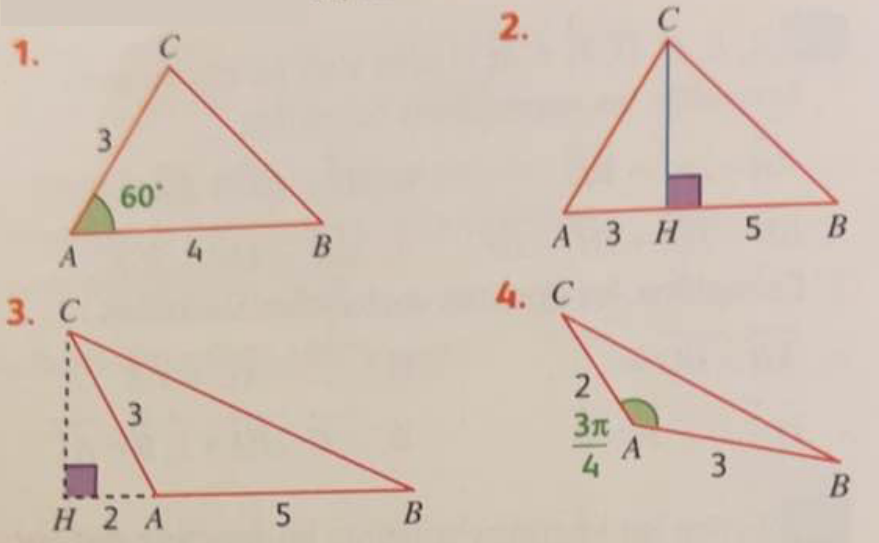
\includegraphics[scale=0.4]{1.04.02-Img03}
\end{center}
\begin{corrBox}
	\begin{enumMet}
		\item $\vv{A B} \cdot \vv{A C}=\vv{A B} \cdot \vv{A H}=-AB\times AH=-5\times2=-10$
		\item $\vv{A B} \cdot \vv{A C}=\vv{A B} \cdot \vv{A H}=AB\times AH=8\times3=24$
	\end{enumMet}
\end{corrBox}




\end{document}

